%Version 3.1 December 2024
% See section 11 of the User Manual for version history
%%%%%%%%%%%%%%%%%%%%%%%%%%%%%%%%%%%%%%%%%%%%%%%%%%%%%%%%%%%%%%%%%%%%%%
%%                                                                 %%
%% Please do not use \input{...} to include other tex files.       %%
%% Submit your LaTeX manuscript as one .tex document.              %%
%%                                                                 %%
%% All additional figures and files should be attached             %%
%% separately and not embedded in the \TeX\ document itself.       %%
%%                                                                 %%
%%%%%%%%%%%%%%%%%%%%%%%%%%%%%%%%%%%%%%%%%%%%%%%%%%%%%%%%%%%%%%%%%%%%%
%%\documentclass[referee,sn-basic]{sn-jnl}% referee option is meant for double line spacing

%%=======================================================%%
%% to print line numbers in the margin use lineno option %%
%%=======================================================%%

%%\documentclass[lineno,pdflatex,sn-basic]{sn-jnl}% Basic Springer Nature Reference Style/Chemistry Reference Style

%%=========================================================================================%%
%% the documentclass is set to pdflatex as default. You can delete it if not appropriate.  %%
%%=========================================================================================%%

%%\documentclass[sn-basic]{sn-jnl}% Basic Springer Nature Reference Style/Chemistry Reference Style
%%Note: the following reference styles support Namedate and Numbered referencing. By default the style follows the most common style. To switch between the options you can add or remove �Numbered� in the optional parenthesis.
%%The option is available for: sn-basic.bst, sn-chicago.bst%

\documentclass[pdflatex,sn-nature,lineno]{sn-jnl}% Style for submissions to Nature Portfolio journals
%\documentclass[pdflatex,sn-basic]{sn-jnl}% Basic Springer Nature Reference Style/Chemistry Reference Style
%\documentclass[pdflatex,sn-mathphys-num]{sn-jnl}% Math and Physical Sciences Numbered Reference Style
%\documentclass[pdflatex,sn-mathphys-ay]{sn-jnl}% Math and Physical Sciences Author Year Reference Style
%\documentclass[pdflatex,sn-aps]{sn-jnl}% American Physical Society (APS) Reference Style
%\documentclass[pdflatex,sn-vancouver-num]{sn-jnl}% Vancouver Numbered Reference Style
%\documentclass[pdflatex,sn-vancouver-ay]{sn-jnl}% Vancouver Author Year Reference Style
%\documentclass[pdflatex,sn-apa]{sn-jnl}% APA Reference Style
%\documentclass[pdflatex,sn-chicago]{sn-jnl}% Chicago-based Humanities Reference Style

%%%% Standard Packages
%%<additional latex packages if required can be included here>
\usepackage{graphicx}%
\usepackage{multirow}%
\usepackage{amsmath,amssymb,amsfonts}%
\usepackage{amsthm}%
\usepackage{mathrsfs}%
\usepackage[title]{appendix}%
\usepackage{xcolor}%
\usepackage{textcomp}%

% Define argmax operator
\DeclareMathOperator*{\argmax}{argmax}
\usepackage{manyfoot}%
\usepackage{booktabs}%
\usepackage{algorithm}%
\usepackage{algorithmicx}%
\usepackage{algpseudocode}%
\usepackage{listings}%

% \usepackage{caption}
\usepackage{standalone}
\usepackage{tikz}
\usepackage[dvipsnames]{xcolor}
\usepackage{geometry}
\usepackage{textcomp} % using \textquotesingle
% Minted package for beautiful syntax highlighting
\usepackage{minted}
\usemintedstyle{borland}
\setminted{
  fontsize=\small,
  breaklines=true,
  autogobble,
  frame=single,
  framesep=2mm,
  linenos
}

% Use bash lexer for TSG code examples (since it handles # comments well)
\newminted{bash}{
  fontsize=\small,
  breaklines=true,
  autogobble,
  frame=single,
  framesep=2mm,
  linenos
}

\usetikzlibrary{shadows,shapes,arrows,positioning,fit,backgrounds,decorations.pathreplacing,calc}

\graphicspath{{../figures}}

\usepackage[acronym, automake, style=index, shortcuts]{glossaries-extra}
\setabbreviationstyle[acronym]{long-short}
% define glossaries
\makeglossaries

\newacronym{wga}{WGA}{whole genome amplification}
\newacronym{wgs}{WGS}{whole genome sequencing}
\newacronym{mda}{MDA}{multiple displacement amplification}
\newacronym{malbac}{MALBAC}{multiple annealing and looping-based amplification cycles}

\newacronym{gpu}{GPU}{graphics processing unit}
\newacronym{cpu}{CPU}{central processing unit}
\newacronym{hpc}{HPC}{high performance computing}

\newacronym{sv}{SV}{structural variation}
\newacronym{snp}{SNP}{single nucleotide polymorphism}

\newacronym{ont}{ONT}{Oxford Nanopore Technologies}
\newacronym{pb}{PacBio}{Pacific Biosciences}

\newacronym{del}{DEL}{deletion}
\newacronym{dup}{DUP}{duplication}
\newacronym{ins}{INS}{insertion}
\newacronym{inv}{INV}{inversion}
\newacronym{tra}{TRA}{translocation}

\newacronym{pcr}{PCR}{polymerase chain reaction}
\newacronym{mrna}{mRNA}{messenger RNA}
\newacronym{facs}{FACS}{fluorescence-activated cell sorting}
\newacronym{sa}{SA}{supplementary alignment}

\newacronym{lianti}{LIANTI}{linear amplification via transposon insertion}
\newacronym{doppcr}{DOP-PCR}{degenerate oligonucleotide-primed PCR}
\newacronym{pta}{PTA}{primary template-directed amplification}
\newacronym{dmda}{dMDA}{droplet-based MDA}

\newacronym{ide}{IDE}{integrated development environment}
\newacronym{cd}{CD}{continuous development}
\newacronym{ucsc}{UCSC}{UCSC Genome Browser}

\newacronym{glm}{GLM}{genomic language model}
\newacronym{lcglm}{LCGLM}{long-context genomic language model}
\newacronym{mlp}{MLP}{multilayer perceptron}
\newacronym{gelu}{GELU}{Gaussian error linear unit}


%%%%%=============================================================================%%%%
%%%%  Remarks: This template is provided to aid authors with the preparation
%%%%  of original research articles intended for submission to journals published
%%%%  by Springer Nature. The guidance has been prepared in partnership with
%%%%  production teams to conform to Springer Nature technical requirements.
%%%%  Editorial and presentation requirements differ among journal portfolios and
%%%%  research disciplines. You may find sections in this template are irrelevant
%%%%  to your work and are empowered to omit any such section if allowed by the
%%%%  journal you intend to submit to. The submission guidelines and policies
%%%%  of the journal take precedence. A detailed User Manual is available in the
%%%%  template package for technical guidance.
%%%%%=============================================================================%%%%

%% as per the requirement new theorem styles can be included as shown below
\theoremstyle{thmstyleone}%
\newtheorem{theorem}{Theorem}%  meant for continuous numbers
%%\newtheorem{theorem}{Theorem}[section]% meant for sectionwise numbers
%% optional argument [theorem] produces theorem numbering sequence instead of independent numbers for Proposition
\newtheorem{proposition}[theorem]{Proposition}%
%%\newtheorem{proposition}{Proposition}% to get separate numbers for theorem and proposition etc.

\theoremstyle{thmstyletwo}%
\newtheorem{example}{Example}%
\newtheorem{remark}{Remark}%

\theoremstyle{thmstylethree}%
\newtheorem{definition}{Definition}%

\raggedbottom
%%\unnumbered% uncomment this for unnumbered level heads

\begin{document}

\title[Article Title]{ChimeraLM: A genomic language model that distinguishes true structural variants from artifacts in whole-genome amplification–based long-read sequencing}

%%=============================================================%%
%% GivenName	-> \fnm{Joergen W.}
%% Particle	-> \spfx{van der} -> surname prefix
%% FamilyName	-> \sur{Ploeg}
%% Suffix	-> \sfx{IV}
%% \author*[1,2]{\fnm{Joergen W.} \spfx{van der} \sur{Ploeg}
%%  \sfx{IV}}\email{iauthor@gmail.com}
%%=============================================================%%
\author[1]{\fnm{Yangyang} \sur{Li}}\email{yangyang.li@northwestern.edu}
\equalcont{These authors contributed equally to this work.}
\author[1]{\fnm{Qingxiang} \sur{Guo}}\email{qingxiang.guo@northwestern.edu}
\equalcont{These authors contributed equally to this work.}
\author*[1,2]{\fnm{Rendong} \sur{Yang}}\email{rendong.yang@northwestern.edu}

\affil[1]{\orgdiv{Department of Urology}, \orgname{Northwestern University Feinberg School of Medicine}, \orgaddress{\street{303 E Superior St}, \city{Chicago}, \postcode{60611}, \state{IL}, \country{USA}}}
\affil[2]{\orgdiv{Robert H. Lurie Comprehensive Cancer Center}, \orgname{Northwestern University Feinberg School of Medicine}, \orgaddress{\street{675 N St Clair St}, \city{Chicago}, \postcode{60611}, \state{IL}, \country{USA}}}

\abstract{Single-cell genomic analysis relies on \gls{wga} to generate sufficient DNA for sequencing, yet this process introduces chimeric artifacts that manifest as false-positive \gls{sv} and compromise downstream analyses. Here we present ChimeraLM, a \gls{glm} that identifies \gls{wga}-induced chimeric artifacts directly from sequence information. ChimeraLM is trained on matched \gls{wga} and bulk sequencing from the same sample, using bulk support to label chimeric reads as amplification-induced artifacts or genuine events. To capture long-range dependencies in variable-length reads, the model combines Hyena operators with attention pooling. Evaluated on matched \gls{wga} and bulk nanopore datasets, ChimeraLM reduced chimeric reads by ${\sim}$90\%, restoring chimeric rates to near-bulk levels, whereas existing methods achieved at most 8\% reduction. When applied to \gls{sv} calling, ChimeraLM reduced false-positive calls by 8–11 fold while retaining 72–92\% of bulk-supported variants. ChimeraLM further normalized \gls{sv}-type distributions toward bulk profiles by suppressing the characteristic \gls{inv} bias observed in unprocessed \gls{wga} data. Attention-based interpretation indicates that ChimeraLM concentrates classification evidence at chimeric junctions, demonstrating capacity to learn biologically interpretable features. ChimeraLM provides a general approach for suppressing amplification-induced artifacts, enabling more reliable single-cell \gls{sv} analysis across long-read platforms.}
\keywords{Whole Genome Amplification, Single Cell, Genomic Language Model, Structural Variation}

\maketitle

% It resets the counters so the Main section treats acronyms as new.
\glsresetall

\section*{Main}\label{sec:main}

Single-cell and low-input genomics have transformed our ability to resolve biological heterogeneity, enabling the discovery of rare cell states and the reconstruction of clonal evolution in cancer and development~\cite{kalef2024single,navin2011tumour,sun2024mapping}.
However, the limited DNA input (on the order of picograms per cell) makes comprehensive genome-wide profiling technically challenging~\cite{gawad2016single,chen2017singlecell}.
\Gls{wga} therefore remains a prerequisite for high-coverage sequencing~\cite{macaulay2014single,de2014quantitative,biezuner2021comparison}, yet it introduces systematic errors that compromise genomic fidelity, particularly for \gls{sv} detection~\cite{lu2023chimera,lasken2007mechanism,agyabeng2025evaluating}.

A prominent source of error is amplification-induced chimera formation. In WGA methods such as \gls{mda}, highly processive polymerases such as phi29 can switch templates and join discontinuous genomic loci into a single molecule~\cite{dean2002comprehensive,lu2023chimera,lu2023exploration,lasken2007mechanism,agyabeng2025evaluating}.
This problem is particularly consequential for long-read sequencing, which is otherwise well suited for resolving complex \glspl{sv}. Chimeric reads can constitute a substantial fraction of \gls{wga} data~\cite{lu2023chimera}, generating alignment patterns that resemble genuine \glspl{tra} and \glspl{inv}~\cite{lasken2007mechanism}.
Consequently, \gls{sv} callers that rely on alignment-based signals (for example, split-read and supplementary alignments) and coverage-derived evidence frequently misinterpret amplification artifacts as true rearrangements, inflating false positives and distorting \gls{sv} spectra~\cite{Sedlazeck2018,Smolka2024,chen2023deciphering,heller2019svim,jiang2020longreadbased,gonzalez-pena2021accurate,kosugi2019comprehensive,alkan2011genome}.

Distinguishing genuine genomic rearrangements from amplification artifacts remains a major computational challenge.
Existing quality-control approaches typically rely on handcrafted rules or alignment-derived features, such as read orientation signatures or local coverage deviations~\cite{kiguchi2021longread,lu2023exploration,agyabeng2025evaluating}.
However, these heuristics are often sensitive to platform- and protocol-specific variation. Moreover, they cannot capture sequence-level patterns at chimeric junctions or long-range dependencies within reads. As a result, low-input long-read sequencing remains difficult to deploy in settings where high precision is essential, including somatic mosaicism profiling and validation of CRISPR off-target effects.

To address this challenge, we present ChimeraLM, an interpretable \gls{glm} for identifying and filtering \gls{wga}-induced artifacts at the single-read level. Unlike traditional approaches that rely on handcrafted rules derived from read alignments or sequence-level, ChimeraLM formulates artifact detection as a sequence-modeling task and learns discriminative features directly from raw DNA reads~\cite{li2024deepchopper}.
Building on advances in DNA foundation models~\cite{nguyen2023hyenadna,dalla2025nucleotide,zhou2023dnabert,consens2023transformers}, it captures latent motifs and structural dependencies that generalize across nanopore platforms.
Across nanopore \gls{wga} datasets, ChimeraLM reduces chimeric reads by ${\sim}90\%$ while preserving 72--92\% of bulk-supported \glspl{sv}, improving \gls{sv} validation rates by 8.5- to 11.0-fold and restoring bulk-like \gls{sv}-type distributions.
By enabling reliable \gls{sv} discovery in long-read sequencing, ChimeraLM removes a critical data-quality barrier for single-cell genomics.


\section*{Results}\label{sec:results}

\begin{figure}[p]
	\begin{center}
		\includegraphics[width=\textwidth]{final_figures/figure1}
	\end{center}
	\caption{{\bf ChimeraLM workflow and architecture for detecting \gls{wga} artifacts.}
	\textbf{(a)}~Single-cell genomic workflow and ChimeraLM integration. Single cells are isolated, followed by DNA extraction and \gls{wga}. During amplification, chimeric artifacts (red) are generated alongside biological reads (green). After base calling and mapping, ChimeraLM classifies chimeric reads as biological or artificial, enabling downstream \gls{sv} detection on filtered data.
	\textbf{(b)}~Ground truth label generation. Chimeric reads from \gls{wga} data are compared against chimeric reads from bulk sequencing of the same cell line. Reads matching bulk data are labeled biological (green); non-matching reads are labeled artificial (red).
	\textbf{(c)}~ChimeraLM architecture. Input DNA sequences (batch size $B$, sequence length $L$) are tokenized at single-nucleotide resolution and encoded into hidden states $\mathbf{H} \in \mathbb{R}^{L \times 256}$ through DNA encoder (HyenaDNA~\cite{nguyen2023hyenadna}). Hyena operators capture long-range dependencies. Attention pooling aggregates position-specific features, and \gls{mlp} layers with residual connections process pooled representations for binary classification.
	\textbf{(d)}~Attention pooling mechanism. Attention weights $\boldsymbol{\alpha} \in \mathbb{R}^{L \times 1}$ are computed through linear layers with GELU activation and softmax normalization, assigning importance scores to each position. The weighted sum produces a fixed-dimensional representation $\mathbf{h}_{\text{pooled}} \in \mathbb{R}^{256}$.
	Created with BioRender.com.}
	\label{fig:figure1}
\end{figure}

\subsection*{Overview of ChimeraLM workflow and model architecture}

Single-cell long-read genomics requires \gls{wga} to obtain sufficient DNA for sequencing (Fig.~\ref{fig:figure1}a).
However, \gls{wga} introduces artifacts that generate chimeric reads composed of segments from distant genomic loci, which can confound \gls{sv} detection.
ChimeraLM integrates into this workflow as a post-alignment filtering module (Fig.~\ref{fig:figure1}a).
It evaluates each chimeric read prior to variant calling, predicting whether the sequence reflects a genuine genomic rearrangement or a \gls{wga}-induced artifact.
This binary classification enables the selective removal of false positives while preserving authentic biological signal.

To train and evaluate the model, we constructed a high-confidence labeled dataset using two \gls{wga} datasets generated from the same monoclonal PC3 lineage on independent \gls{ont} platforms.
The \gls{ont} PromethION \gls{wga} dataset was designated for model training, whereas the \gls{ont} MinION \gls{wga} dataset was reserved exclusively for the generalization test.
For supervised labeling, chimeric reads from the PromethION \gls{wga} dataset were compared against unamplified bulk DNA sequenced on three long-read platforms (\gls{ont} PromethION, \gls{ont} MinION, and \gls{pb} (see \hyperref[sec:methods]{Methods}; Fig.~\ref{fig:figure1}b; Extended Data Fig.~\ref{fig:data_construction}a)).
\gls{wga} reads were labeled biological if their chimeric structures were supported by any bulk dataset, and artificial if they were absent from all bulk references.

This labeling procedure yielded two groups of \gls{wga} chimeric reads (Extended Data Fig.~\ref{fig:data_construction}b).
Most reads, 12,670,396 in total, showed no supporting alignments in any bulk dataset and were classified as artificial.
The remaining 293,180 reads had at least one matching breakpoint in bulk sequencing, providing evidence that they represent biological rearrangements rather than amplification artifacts.
To construct the supervised training dataset, we retained all 293,180 biological reads and selected an equal number of artificial reads through random subsampling.
We further expanded the biological class by adding 178,748 chimeric reads sampled directly from bulk sequencing data, which represent genuine structural rearrangements independent of \gls{wga}-induced artifacts.
This augmentation ensures that the classifier is exposed to a broader spectrum of true biological chimeric structures.
The final labeled dataset (765,108 reads) was split into training (70\%), validation (20\%), and test (10\%) sets using stratified sampling.

Effective classification of \gls{wga} chimeric reads requires a model that can process long, variable-length DNA sequences while retaining single-nucleotide resolution (Fig.~\ref{fig:figure1}c).
ChimeraLM addresses these challenges through a sequence encoder based on HyenaDNA~\cite{nguyen2023hyenadna}, a genomic foundation model pre-trained on diverse DNA sequences.
Input reads are tokenized at single-nucleotide resolution and processed by Hyena operators~\cite{Poli2023HyenaHT}, which are designed to model long-range dependencies on long reads while still allowing full-length analysis without splitting the sequence.
The encoder outputs a matrix of hidden states across the read.
To obtain a fixed-length representation, an attention-pooling module (Fig.~\ref{fig:figure1}d) assigns learned, position-specific weights and computes a weighted sum over the sequence.
The pooled vector is then processed by \gls{mlp} blocks with residual connections, and a final softmax layer outputs the probability that each read is biological or artificial.

\begin{figure}[!ht]
	\begin{center}
		\includegraphics[width=0.95\textwidth]{final_figures/figure2}
	\end{center}
	\caption{{\bf ChimeraLM accurately identifies and removes \gls{wga}-induced chimeric artifacts.}
		\textbf{(a)}~Classification performance on held-out test data. ChimeraLM achieves recall of 0.95, precision of 0.70, and F1 score of 0.81.
		\textbf{(b)}~Chimeric read reduction across sequencing platforms. Stacked bars show proportions of chimeric (dark teal) and non-chimeric (light teal) reads in bulk, \gls{wga}, and ChimeraLM-filtered samples. ChimeraLM reduces chimeric read frequencies from 46.0\% to 4.9\% (PromethION) and from 23.0\% to 1.5\% (MinION), approaching bulk levels (2.3\% and 2.5\%, respectively).
		\textbf{(c,d)}~Benchmarking against existing methods on PromethION (c) and MinION (d).
		The bar represents the total count of chimeric reads.
		ChimeraLM achieves approximately 90\% reduction in chimeric reads on both platforms; SACRA and 3rd-ChimeraMiner show no detectable reduction.
	}\label{fig:figure2}
\end{figure}

\subsection*{ChimeraLM achieves high accuracy and reduces artifacts to near-bulk levels across platforms}

We first evaluated ChimeraLM on the held-out test set derived from the labeled dataset (Fig.~\ref{fig:figure2}a; see \hyperref[sec:methods]{Methods}).
This test set comprises chimeric reads with known biological or artificial status based on the ground-truth labeling procedure described above.
On this benchmark, ChimeraLM achieved an F1 score of 0.81, with a recall of 0.95 and a precision of 0.70.
The high recall indicates that 95\% of artificial chimeric reads were correctly identified and removed, which is critical for minimizing downstream false-positive \gls{sv} calls, while the precision confirms that most flagged reads correspond to true artifacts rather than biological rearrangements.

We next asked whether ChimeraLM filtering could restore chimeric read rates in full PC3 \gls{wga} datasets to bulk baselines on both PromethION and MinION platforms (Fig.~\ref{fig:figure2}b).
Bulk sequencing established low baseline chimeric read rates of 2.3\% (PromethION) and 2.5\% (MinION).
In contrast, \gls{wga} increased the chimeric fraction to 46.0\% and 23.0\%, respectively.
After ChimeraLM filtering, chimeric content dropped to 4.9\% on PromethION and 1.5\% on MinION, corresponding to 10- to 15-fold reductions, while retaining 15.8 million and 5.6 million biological reads.
These post-filtering rates approach bulk baselines, indicating effective removal of \gls{wga}-induced artifacts while preserving authentic biological signal.

We benchmarked ChimeraLM against SACRA~\cite{kiguchi2021longread} and 3rd-ChimeraMiner~\cite{lu2023exploration}, two existing tools for detecting amplification-induced chimeras (Fig.~\ref{fig:figure2}c,d).
ChimeraLM achieved approximately 90\% reduction in chimeric reads on both platforms, whereas neither SACRA nor 3rd-ChimeraMiner produced a detectable reduction (0\%).

The MinION results are particularly informative because this platform was never used during model training.
ChimeraLM was trained exclusively on PromethION \gls{wga} data, yet achieved comparable chimeric read reduction on MinION.
This cross-platform generalization indicates that ChimeraLM captures sequence-level features intrinsic to \gls{wga}-induced artifacts rather than platform-specific signatures, supporting its potential applicability to additional long-read and short-read sequencing technologies.

% \subsection*{ChimeraLM dramatically outperforms existing chimera detection methods on long-read WGA data}
% P2 92
%
% mk1c 91


\begin{figure}[H]
	\begin{center}
		\includegraphics[width=0.95\textwidth]{final_figures/figure3}
	\end{center}
	\caption{{\bf ChimeraLM improves structural variant detection accuracy.}
		\textbf{(a)}~Construction of a high-confidence \gls{sv} reference dataset from bulk PC3 sequencing. Four bulk datasets were integrated: \gls{ont} MinION Mk1C, \gls{ont} PromethION P2, the CCLE Illumina \gls{wgs} dataset, and the PRJNA361315 Illumina \gls{wgs} dataset. \glspl{sv} were called independently within each dataset using multiple callers, and events supported by $\geq$2 callers per dataset were retained. \glspl{sv} were then compared across datasets, and events observed in $\geq$2 of the four bulk datasets were designated as gold-standard \glspl{sv}.
		\textbf{(b,c)}~\gls{sv} validation against the gold-standard reference for PromethION (b) and MinION (c).
		Bars show \gls{sv} calls supported by the gold standard (dark teal) or unsupported (light teal).
		\textbf{(d,e)}~\gls{sv} validation against platform-matched long-read bulk sequencing for PromethION (d) and MinION (e), capturing true long-read \glspl{sv} that may not be represented in the multi-platform reference.
		Bars show \gls{sv} calls supported by the platform-matched long-read bulk data (dark teal) or unsupported (light teal).
		\textbf{f}~\gls{sv} type distributions for PromethION across bulk, unfiltered \gls{wga}, and \gls{wga}+ChimeraLM.
		Unfiltered \gls{wga} shows an excess of \glspl{inv}, which is reduced after ChimeraLM filtering.
		\textbf{g}~Composition of artifact-supported \glspl{sv} for PromethION. Donut charts summarize \gls{sv} types among events supported exclusively by chimeric reads, representing artificial \glspl{sv} preferentially removed by ChimeraLM.
	}\label{fig:figure3}
\end{figure}

\subsection*{ChimeraLM substantially reduces unsupported structural variant calls}

Accurate \gls{sv} detection from single cells is essential for understanding genomic diversity and disease mechanisms.
However, \gls{wga}-induced chimeric artifacts can be misidentified as genuine \glspl{sv}, leading to incorrect biological conclusions.
To quantify ChimeraLM’s impact on \gls{sv} calling, we compared \gls{sv} callsets generated from unfiltered \gls{wga} reads with those generated after ChimeraLM filtering (\gls{wga} + ChimeraLM).
We evaluated both callsets against two complementary references (Fig.~\ref{fig:figure3}):
(i) a stringent gold-standard \gls{sv} set derived from bulk PC3 DNA by cross-dataset consensus (Fig.~\ref{fig:figure3}a), and
(ii) platform-matched long-read bulk \gls{sv} callsets used as a platform-specific reference for recall (Fig.~\ref{fig:figure3}d,e).

We first constructed a high-confidence gold-standard \gls{sv} set from bulk PC3 DNA using four independent sequencing datasets: \gls{ont} PromethION, \gls{ont} MinION, and two Illumina whole-genome datasets (the CCLE PC3 \gls{wgs} dataset and PRJNA361315 PC3 \gls{wgs} dataset) (Fig.~\ref{fig:figure3}a; Extended Data Table~\ref{tab:seq_stats}).
\glspl{sv} were called separately within each dataset using multiple \gls{sv} callers.
Events supported by at least two callers within a dataset were retained, and only \glspl{sv} observed in at least two of the four datasets were kept as gold-standard events.

Relative to this stringent gold standard, unfiltered \gls{wga} produced extensive unsupported \glspl{sv} (Fig.~\ref{fig:figure3}b,c).
On PromethION, \gls{wga} yielded 3,601,099 \gls{sv} calls, of which only 8,815 (0.24\%) overlapped gold-standard events.
After ChimeraLM filtering, total calls dropped to 305,570 while retaining 8,067 gold-standard events (91.5\% retention), increasing the validation rate to 2.64\% (11-fold) (Fig.~\ref{fig:figure3}b).
On MinION, calls decreased from 451,390 to 38,432, while gold-standard-supported events decreased from 7,193 to 6,269, corresponding to 87.2\% retention.
The validation rate increased from 1.59\% to 16.3\% (10-fold) (Fig.~\ref{fig:figure3}c).

Because the gold standard is intentionally stringent and may miss true \glspl{sv} detectable only in long-read data, we next performed platform-matched validation using long-read bulk sequencing from the same platform (Fig.~\ref{fig:figure3}d,e).
This analysis provides a platform-specific estimate of recall and reduces bias introduced by the strict gold-standard definition.
ChimeraLM increased validation rates from 0.38\% to 3.24\% on PromethION (8.5-fold) and from 1.25\% to 12.79\% on MinION (10-fold), while retaining 71.9\% and 87.1\% of bulk-supported events, respectively.
Together, these results show that ChimeraLM removes an order of magnitude of unsupported \gls{sv} calls while preserving the majority of bulk-supported variants across platforms.

\subsection*{ChimeraLM restores bulk-like SV-type distributions}

Amplification artifacts can distort the apparent spectrum of \glspl{sv}.
We therefore compared \gls{sv} type distributions across bulk, unfiltered \gls{wga}, and ChimeraLM-filtered datasets on both nanopore platforms (Fig.~\ref{fig:figure3}f; Extend Data Fig.~\ref{fig:minion_sv_distribution}).
Bulk sequencing showed a balanced mixture of \glspl{del}, \glspl{dup}, \glspl{ins}, \glspl{inv}, and \glspl{tra}.
In contrast, unfiltered \gls{wga} callsets were dominated by \glspl{inv} on both platforms.
After ChimeraLM filtering, excessive \glspl{inv} were markedly reduced, and the overall \gls{sv} type profile shifted toward the bulk distribution, while the relative proportions of other \gls{sv} classes remained largely stable.

To identify which \gls{sv} types were primarily driven by \gls{wga}-induced artifacts, we examined \gls{sv} calls supported exclusively by reads classified as chimera artifacts (Fig.~\ref{fig:figure3}g; Extend Data Fig.~\ref{fig:minion_sv_artifact_distribution}).
These artifact-supported events were overwhelmingly \glspl{inv}, accounting for 88.4\% on PromethION and 92.4\% on MinION.
The remaining calls included smaller fractions of \glspl{del} (5.1\% and 3.8\%), \glspl{dup} (3.4\% and 2.4\%), and \glspl{ins} (3.0\% and 1.4\%), indicating that \gls{wga}-induced chimeras can generate false positives across multiple \gls{sv} categories.

Together, these results show that \gls{wga} artifacts preferentially inflate \glspl{inv} but are not limited to a single \gls{sv} class.
By selectively removing artifact-supported events and restoring \gls{sv} type distributions toward bulk-like patterns, ChimeraLM improves the robustness and interpretability of single-cell \gls{sv} analyses.


\begin{figure}[H]
	\begin{center}
		\includegraphics[width=\textwidth]{final_figures/figure4}
	\end{center}
	\caption{{\bf ChimeraLM attention weights are enriched at chimeric junction regions.}
		\textbf{(a,b)}~Attention weight profiles for two representative chimeric reads exhibiting distinct junction configurations.
		Upper panels show per-position attention weights (blue) with the mean attention across the read indicated by a dashed line.
		Red vertical lines mark inferred chimeric junction positions, and pink shading denotes the junction-centered region ($\pm$50~bp).
		Lower panels display read-level alignments, highlighting orientation transitions at the junctions (green, forward orientation; red, reverse-complemented orientation).
		\textbf{(c,d)}~Quantitative comparison of attention weights between junction and non-junction regions.
		Junction-centered windows show significantly elevated attention weights relative to non-junction regions ($P = 5.3 \times 10^{-14}$ and $P = 6.8 \times 10^{-15}$; Wilcoxon rank-sum test).
		\textbf{(e,f)}~Schematic illustration of \gls{wga}-induced chimera formation.
		During amplification, DNA fragments originating from distant genomic loci can be amplified in either orientation, joining them into a single molecule with discordant orientations, producing \gls{inv}-like alignment signatures.
		The two examples illustrate forward-to-reverse and reverse-to-forward orientation transitions.
	}\label{fig:figure4}
\end{figure}


\subsection*{Attention visualization reveals interpretable classification features}

We examined whether ChimeraLM’s attention weights provide an interpretable signal by focusing on mechanistically relevant regions of chimeric reads, particularly the junctions during \gls{wga} (Fig.~\ref{fig:figure4}).
We inspected two representative chimeric reads exhibiting distinct junction configurations (Fig.~\ref{fig:figure4}a,b).
In both cases, attention remained relatively flat across most positions but formed sharp, concentrated peaks at the inferred junction regions.
These peaks aligned with the read-level breakpoint separating two genomic loci and coincided with an orientation transition between adjacent alignment segments.

To quantify this effect, we compared attention weights within junction-centered windows ($\pm$50~bp) against weights from non-junction regions (Fig.~\ref{fig:figure4}c,d).
Junction windows showed significantly higher attention weights (Wilcoxon rank-sum test, $P = 5.3 \times 10^{-14}$ and $P = 6.8 \times 10^{-15}$), indicating that ChimeraLM preferentially emphasizes sequence context proximal to chimeric junctions.

This attention enrichment is consistent with the expected structure of \gls{wga}-induced chimeras (Fig.~\ref{fig:figure4}e,f): DNA fragments from distant loci can be amplified in either orientation and subsequently joined, generating junctions with discordant orientations.
Together, these results suggest that ChimeraLM’s attention peaks provide a mechanistically interpretable signal that concentrates classification evidence to junction-proximal sequence positions within individual reads.

\section*{Discussion}\label{sec:discussion}

\gls{wga} enables genomic analysis from single cells but introduces chimeric artifacts that compromise \gls{sv} detection.
ChimeraLM addresses this challenge by classifying chimeric reads as biological or artificial from sequence information and filtering \gls{wga}-induced artifacts before variant calling, rather than attempting to correct artifact-driven calls post hoc.
Across nanopore platforms, ChimeraLM yielded consistent improvements at both read and variant levels.
It reduced chimeric reads by \(\sim\)90\% while retaining 72--92\% of bulk-supported \glspl{sv}, and it lowered unsupported \gls{sv} calls by 8.5--11.0 fold.
Performance generalized from PromethION (used for training) to MinION without platform-specific retraining, indicating that ChimeraLM captures properties shared by \gls{wga}-induced artifacts rather than instrument-specific signatures.
In contrast, SACRA and 3rd-ChimeraMiner failed to reduce chimeric content on our long-read \gls{wga} datasets, underscoring the limitations of heuristic strategies and indicating the need for models that learn discriminative features directly from sequence data.

The efficacy of ChimeraLM highlights the utility of deep learning in quality control tasks where conventional metrics (e.g., mapping quality, read depth) provide limited resolution~\cite{lu2023exploration,kiguchi2021longread,li2024deepchopper}.
By learning directly from sequence data, ChimeraLM discovers subtle compositional and structural features that differentiate authentic sequences from amplification artifacts.
The model also offers interpretability through attention visualization: attention weights concentrate at junction regions where template switching joins discordant loci, validating the biological relevance of the learned features.
These methodological advances have direct implications for single-cell genomics, where high false-positive rates in \gls{wga} data have constrained robust characterization of chromosomal instability, clonal evolution, and \gls{sv} burden~\cite{kosugi2019comprehensive,mahmoud2019structural}.
By improving the signal-to-noise ratio and clarifying \gls{sv}-type spectra that are otherwise distorted by amplification artifacts, ChimeraLM enables more confident identification of genuine \glspl{sv}, supporting studies of cancer evolution, developmental biology, and somatic mosaicism where single-cell resolution is essential.

Several limitations warrant consideration.
First, the current model processes reads independently; integrating contextual features such as coverage or phasing information may further enhance accuracy. Second, regarding computational resources, while \gls{cpu} inference is feasible, \gls{gpu} acceleration is recommended for processing large-scale datasets.
Finally, future work should extend validation to diverse cell types, sequencing platforms (e.g., PacBio HiFi), and alternative \gls{wga} protocols—including \gls{malbac}~\cite{zong2012genome}, \gls{lianti}~\cite{chen2017singlecell}, \gls{pta}~\cite{gonzalez-pena2021accurate}, and \gls{dmda}~\cite{dippenaar2024droplet}.
Although the sequence-level approach implies effective transferability, such broad validation is essential to optimize performance across specific amplification chemistries.

Broadly, ChimeraLM illustrates the potential of \glspl{glm} for genomic data quality control.
With emerging long-context architectures~\cite{nguyen2023hyenadna}, the model's context window could be extended to 1M tokens, enabling analysis of increasingly complex genomic structures.
This framework could extend to other amplification-dependent technologies, such as cell-free DNA analysis, ancient DNA studies, and metagenomics from low-biomass samples.
Furthermore, attention-based interpretability opens opportunities for studying template-switching dynamics, potentially guiding the development of improved amplification protocols.
In summary, ChimeraLM provides a practical and interpretable framework for enhancing long-read single-cell genomic fidelity, ensuring that downstream biological insights are derived from genuine \glspl{sv} rather than technical artifacts.

\section*{Methods}\label{sec:methods}

\subsection*{Cell culture, single-clone preparation, and nanopore sequencing}

\paragraph{Cell culture and single-clone establishment}
PC3 prostate cancer cells (ATCC\textsuperscript{\textregistered} CRL-1435\texttrademark) were cultured in RPMI-1640 medium supplemented with 10\% fetal bovine serum and 1\% penicillin--streptomycin at 37~\textdegree C with 5\% CO\textsubscript{2}. To minimize biological heterogeneity, a monoclonal population was established by serial dilution in 96-well plates, ensuring that each culture originated from a single cell. Mycoplasma contamination was routinely tested and confirmed negative prior to DNA extraction.

\paragraph{DNA extraction and whole-genome amplification}
From the monoclonal population, two types of DNA samples were prepared: a bulk (non-amplified) control and ten single-cell MDA-amplified genomes. Bulk high-molecular-weight DNA was extracted using the Monarch\textsuperscript{\textregistered} HMW DNA Extraction Kit for Cells \& Blood (New England Biolabs). Individual cells were isolated using 1CellDish-60~mm (iBiochips) and amplified using the REPLI-g Advanced DNA Single Cell Kit (Qiagen) following the manufacturer's protocol. DNA concentration and fragment integrity were assessed with a Qubit~4 fluorometer and Agilent TapeStation (DNA~1000/5000 ScreenTape). Only samples meeting quality standards were used for library construction.

\paragraph{Nanopore library preparation and sequencing}
Libraries were prepared using the \gls{ont} Ligation Sequencing Kit~V14 (SQK-LSK114) and sequenced on MinION~Mk1C or PromethION~P2~Solo devices with R10.4.1 flow cells following the manufacturer’s genomic DNA workflow. Because all single-cell samples originated from the same monoclonal lineage, differences between amplified and bulk datasets primarily reflect MDA-induced artifacts rather than biological variation.

\paragraph{Basecalling and read processing}
POD5 files were basecalled using Dorado~v0.5.0 with the high-accuracy model \texttt{dna\_r10.4.1\_e8.2\_400bps\_hac@v4.3.0}~\cite{dorado2023}. Reads with mean quality $<10$ or length $<500$~bp were removed. Adapters and concatemers were trimmed using Cutadapt~v4.0~\cite{martin2011cutadapt} in a two-pass, error-tolerant procedure. Filtered reads were aligned to the GRCh38.p13 reference genome using minimap2~v2.26 (\texttt{map-ont} preset)~\cite{li2018minimap2}. BAM files were sorted and indexed using SAMtools~v1.16~\cite{danecek2021twelve}. Read-length and mapping statistics were computed using NanoPlot~v1.46.1~\cite{decoster2023nanopack2}. All samples were processed using identical parameters.

\paragraph{Chimeric read identification}
Chimeric reads were identified from BAM files using \gls{sa} tags.
Reads were classified as chimeric if they (i) were mapped, (ii) contained an \gls{sa} tag, (iii) were primary alignments (not secondary), and (iv) were not supplementary alignments themselves.
This definition counts each chimeric read once using its primary alignment while excluding secondary/supplementary records, thereby avoiding double-counting and reducing ambiguity from low-confidence alignments. Reads lacking \gls{sa} tags were classified as non-chimeric.

\subsection*{Training data construction}

\paragraph{Data generation and sources}
To construct the training dataset, we generated \gls{wga} and bulk sequencing data from PC3 cells.
The \gls{wga} sample was amplified and sequenced on the PromethION P2 platform (\gls{ont}), while three independent bulk datasets were produced from non-amplified genomic DNA: bulk PromethION P2, bulk MinION Mk1c (\gls{ont}), and bulk \gls{pb}.
These bulk datasets represent authentic biological sequences free from amplification-induced artifacts.
In contrast, \gls{wga} sequencing includes both genuine genomic reads and artificial chimeras introduced during the amplification process.

\paragraph{Ground truth annotation and class definition}
Ground truth labels were established by systematically comparing chimeric reads from the \gls{wga} PromethION P2 dataset against those from the three bulk datasets.
For each \gls{wga} chimeric read, all alignment segments---defined by their genomic start and end coordinates---were compared to the corresponding segments of bulk chimeric reads.
A \gls{wga} read was labeled as biological if every segment matched at least one bulk chimeric read within a 1~kb positional tolerance, indicating that the structural configuration is also present in non-amplified DNA.
Reads lacking any matching pattern across all bulk datasets were labeled as artificial chimeras, presumed to arise from the amplification process.
Additional chimeric reads were randomly sampled from the bulk datasets and labeled as biological, as these reads originate from genuine genomic rearrangements such as true \glspl{sv}.
The final labeled dataset combined the annotated \gls{wga} PromethION P2 reads with the subsampled bulk chimeric reads and was subsequently partitioned into training, validation, and test sets as described below.

\paragraph{Dataset partitioning and cross-platform validation}
The combined labeled dataset, derived from \gls{wga} PromethION P2 and bulk sequencing data, was divided into training (70\%), validation (20\%), and test (10\%) sets using stratified random sampling.
These subsets were used respectively for model training, hyperparameter tuning, and performance evaluation on data from the same sequencing platform.

To evaluate cross-platform generalization, the complete \gls{wga} MinION Mk1c dataset was reserved.
This dataset, generated on a different nanopore platform, was never used during model training or internal testing.
This two-level evaluation design allowed us to test whether ChimeraLM captures general sequence features of amplification-induced chimeras rather than platform-specific artifacts.

\subsection*{Model architecture}

\paragraph{DNA encoder}
ChimeraLM employs the pre-trained HyenaDNA model~\cite{nguyen2023hyenadna} as its DNA encoder.
This model was pre-trained on large-scale genomic data and provides robust sequence representations.
DNA sequences are tokenized at single-nucleotide resolution, with each base (A, C, G, T, N) mapped to a unique integer token (7, 8, 9, 10, 11, respectively).
Special tokens include [CLS]=0, [PAD]=4, and others for sequence processing.
Input sequences are truncated at 32,768 bp or padded to enable batch processing.

For a tokenized input sequence $\mathbf{x} \in \mathbb{Z}^{L}$, the HyenaDNA generates contextualized hidden representations:
\[
	\mathbf{H} = \text{HyenaDNA}(\mathbf{x}) \in \mathbb{R}^{L \times 256}
\]
where $\mathbf{H} = (\mathbf{h}_1, \mathbf{h}_2, \ldots, \mathbf{h}_L)$ represents position-wise hidden states with dimension 256.
The Hyena operators~\cite{Poli2023HyenaHT} efficiently capture both local sequence motifs and long-range dependencies essential for distinguishing biological sequences from chimeric artifacts.

\paragraph{Attention pooling}
To aggregate variable-length sequence representations into fixed-size vectors, ChimeraLM implements attention-based pooling.
For hidden states $\mathbf{H} \in \mathbb{R}^{L \times 256}$, attention weights are computed through a two-layer network:
\begin{align*}
	\mathbf{e}          & = \text{GELU}(\text{Linear}_{256 \to 256}(\mathbf{H})) \in \mathbb{R}^{L \times 256} \\
	\mathbf{s}          & = \text{Linear}_{256 \to 1}(\mathbf{e}) \in \mathbb{R}^{L \times 1}                  \\
	\boldsymbol{\alpha} & = \text{softmax}(\mathbf{s}) \in \mathbb{R}^{L \times 1}
\end{align*}
The pooled representation is the weighted sum of hidden states:
\[
	\mathbf{h}_{\text{pooled}} = \sum_{i=1}^{L} \alpha_i \mathbf{h}_i \in \mathbb{R}^{256}
\]
This mechanism assigns learned importance weights to each sequence position, enabling the model to focus on informative regions while accommodating natural variability in read lengths.

\paragraph{Classification head}
The pooled representation is processed through a \gls{mlp} with residual connections.
The first layer expands dimensionality:
\[
	\mathbf{f}_1 = \text{Dropout}_{0.1}(\text{GELU}(\text{Linear}_{256 \to 512}(\mathbf{h}_{\text{pooled}}))) \in \mathbb{R}^{512}
\]
Subsequent residual blocks with input $\mathbf{f}_{\text{in}} \in \mathbb{R}^{512}$ compute:
\[
	\mathbf{f}_{\text{out}} = \text{Dropout}_{0.1}(\text{Linear}_{512 \to 512}(\text{GELU}(\text{Linear}_{512 \to 512}(\mathbf{f}_{\text{in}}))))) + \mathbf{f}_{\text{in}}
\]
where the skip connection enables stable gradient flow during training.
The final layer produces binary classification logits:
\[
	\mathbf{z} = [z_0, z_1] = \text{Linear}_{512 \to 2}(\mathbf{f}_{\text{final}}) \in \mathbb{R}^{2}
\]
where $z_0$ and $z_1$ represent logits for biological and artificial chimeric classes, respectively. During inference, the predicted class is $\hat{y} = \argmax_{i \in \{0,1\}} z_i$.

\paragraph{Model summary}
The complete ChimeraLM pipeline processes DNA sequences through: (1) single-nucleotide tokenization, (2) HyenaDNA backbone encoding to generate contextualized representations, (3) attention pooling to aggregate position-specific features, (4) \gls{mlp} layers with residual connections to learn classification features, and (5) binary classification output.
The entire model is trained end-to-end using labeled data.

\subsection*{Model training and optimization}

\paragraph{Training configuration}
ChimeraLM was trained using PyTorch~\cite{paszke2019pytorch} and PyTorch Lightning~\cite{Falcon_PyTorch_Lightning_2019} frameworks.
Input sequences were tokenized using the tokenizer with maximum sequence length of 32,768 bp.
Sequences longer than this threshold were truncated; shorter sequences were padded to enable batch processing.
Training employed mixed-precision computation (bf16) to accelerate training while maintaining numerical stability.

\paragraph{Optimization procedure}
We used the AdamW optimizer~\cite{loshchilov2017decoupled} with learning rate $\eta = 1 \times 10^{-4}$ and weight decay $\lambda = 0.01$.
AdamW implements adaptive learning rates with decoupled weight decay, combining the benefits of Adam optimization with proper L2 regularization.
A ReduceLROnPlateau scheduler dynamically adjusted the learning rate based on validation loss, reducing it by a factor of 0.1 when no improvement occurred for 10 consecutive epochs.
Early stopping with patience of 10 epochs prevented overfitting by terminating training when validation performance plateaued.
A fixed random seed (12345) ensured reproducibility across training runs.

The training objective used cross-entropy loss for binary classification.
For a training example with class label $y \in \{0,1\}$ and model logits $\mathbf{z} = [z_0, z_1]$, the loss is:
\[
	\mathcal{L}(\mathbf{z}, y) = -\log\left(\frac{\exp(z_y)}{\exp(z_0) + \exp(z_1)}\right) = -z_y + \log(\exp(z_0) + \exp(z_1))
\]
where $z_0$ and $z_1$ represent logits for biological and artificial chimeric classes, respectively.

\paragraph{Training implementation}
Training used batch size of 16 sequences with 30 parallel data loading workers.
\gls{gpu} acceleration was employed for efficient processing, with training typically requiring 55 hours.
Model checkpointing saved the best-performing model based on validation metrics.
Configuration management used Hydra~\cite{Yadan2019Hydra} to enable reproducible experimentation.

\paragraph{Model evaluation}
Performance was monitored using precision, recall, and F1 score on the validation set after each epoch:
\begin{align*}
	\text{Precision} & = \frac{\text{TP}}{\text{TP}+\text{FP}}, \quad
	\text{Recall} = \frac{\text{TP}}{\text{TP}+\text{FN}}                                                        \\
	\text{F1}        & = \frac{2 \times \text{Precision} \times \text{Recall}}{\text{Precision} + \text{Recall}}
\end{align*}
where TP (true positives) are chimeric reads correctly classified as artificial, TN (true negatives) are biological reads correctly classified as biological, FP (false positives) are biological reads misclassified as artificial, and FN (false negatives) are artificial reads misclassified as biological.
Final model selection was based on best validation performance as determined by early stopping.

\subsection*{Model inference and application}

\paragraph{Inference pipeline}
To apply ChimeraLM to new \gls{wga} sequencing data, the model takes a BAM file as input.
Chimeric reads are identified using \gls{sa} tags and filtered to exclude unmapped, secondary, or supplementary alignments.
Each chimeric read sequence is tokenized using the tokenizer (maximum length 32,768 bp, with truncation or padding as needed).
The trained model processes sequences in batches, generating two logits $[z_0, z_1]$ for each read corresponding to biological and artificial chimeric classes.
Classification is determined by $\hat{y} = \argmax(z_0, z_1)$.
ChimeraLM outputs a filtered BAM file containing only reads classified as biological, which can be directly used for downstream analyses including \gls{sv} calling.

\subsection*{Performance evaluation}

\paragraph{Test set evaluation}
Final model performance was evaluated on the held-out test set and the independent MinION Mk1c dataset.
Metrics (precision, recall, and F1 score) were computed as described in the training section, where true positives represent chimeric reads correctly classified as artificial and true negatives represent biological reads correctly classified as biological.

\paragraph{SV calling}
\glspl{sv} were called using multiple tools to ensure comprehensive detection.
For long-read data (\gls{ont} PromethION P2 and MinION Mk1c), we used Sniffles v2.5~\cite{Sedlazeck2018, Smolka2024}, DeBreak v1.2~\cite{chen2023deciphering}, SVIM v2.0.0~\cite{heller2019svim}, and cuteSV v2.1.1~\cite{jiang2020longreadbased}.
For short-read data of the PC3 cell line, we used both the CCLE Illumina \gls{wgs} dataset and the PRJNA361315 Illumina \gls{wgs} dataset, processed with Manta v1.6.0~\cite{chen2016manta}, DELLY v1.5.0~\cite{rausch2012delly}, and SvABA v1.1.0~\cite{wala2018svaba}.
All tools were executed with default recommended parameters.

\paragraph{Gold standard SV dataset construction}
To evaluate the impact of ChimeraLM on \gls{sv} detection accuracy, we generated a high-confidence gold-standard \gls{sv} set from bulk PC3 sequencing data.
All \gls{sv} comparisons and breakpoint corrections were performed using OctopuSV v0.2.3~\cite{guo2025octopusv}.
Four bulk datasets were integrated: \gls{ont} MinION Mk1c, \gls{ont} PromethION P2, the CCLE Illumina \gls{wgs} dataset, and the PRJNA361315 Illumina \gls{wgs} dataset.
\glspl{sv} were called independently within each dataset, and events supported by at least two \gls{sv} callers were retained.
The remaining calls were then compared across datasets, and \glspl{sv} observed in at least two of the four datasets were designated as gold-standard events for benchmarking.

\paragraph{SV benchmarking analysis}
To assess the impact of ChimeraLM on \gls{sv} calling accuracy, we compared \gls{sv} calls from unfiltered \gls{wga} data and ChimeraLM-filtered \gls{wga} data against two references: (1) the stringent multi-platform gold standard dataset, and (2) platform-matched long-read bulk sequencing data.
Benchmarking was performed using Truvari v4.2.2~\cite{english2022truvari} with default parameters.
\glspl{sv} were considered supported if they matched reference variants within the defined breakpoint tolerance.
Validation rates were calculated as the proportion of called \glspl{sv} supported by the reference.
This dual benchmarking strategy quantifies both improvements in detecting high-confidence multi-platform \glspl{sv} and the retention of platform-specific true variants.

\subsection*{Benchmarking against existing methods}
ChimeraLM was compared to two existing computational methods for detecting amplification-induced chimeric artifacts: SACRA~\cite{kiguchi2021longread} (GitHub commit~9a2607e) and 3rd-ChimeraMiner~\cite{lu2023exploration} (GitHub commit~04b5233).
Both tools were applied to \gls{wga} data from PromethION P2 and MinION Mk1c platforms using default parameters as recommended in their documentation.
Performance was evaluated by measuring the percentage reduction in chimeric reads relative to unprocessed \gls{wga} data.
Chimeric reads were identified using \gls{wga} tag-based alignment criteria (reads with \gls{sa} tags indicating split alignments), and reduction rates were calculated as the proportion of chimeric reads removed by each method.

\subsection*{Attention weight analysis}
To investigate ChimeraLM's interpretability, we analyzed attention weights from the pooling mechanism for representative chimeric reads.
Attention weights indicate the relative importance assigned to each sequence position during classification.
For selected reads, we extracted per-position attention weights and visualized them alongside read alignments to identify whether the model focuses on mechanistically relevant regions.

Chimeric junction positions were identified from alignment data (defined by breakpoints in \gls{sa} tags).
A region of $\pm$50 bp surrounding each junction was designated as the junction region.
Attention weights within junction region were compared to non-junction regions using the Wilcoxon rank-sum test~\cite{2020SciPy-NMeth}, with statistical significance assessed at $p < 0.001$.

\subsection*{Data visualization}
Figures were generated using Python with Matplotlib~\cite{Hunter2007} and Seaborn~\cite{Waskom2021}.

\subsection*{Computing resources}
Computations were performed on a \gls{hpc} server with 64-core Intel Xeon Gold 6338 CPU, 256 GB RAM, and two NVIDIA A100 \glspl{gpu} (80 GB memory each).

\backmatter

\bmhead{Supplementary information}

\makeatletter
\renewcommand{\theHfigure}{extended.\thefigure}
\renewcommand{\theHtable}{extended.\thetable}
\makeatother

\renewcommand{\figurename}{Extended Data Fig.}
\renewcommand{\tablename}{Extended Data Table}
\setcounter{figure}{0}
\setcounter{table}{0}

\begin{table}[!ht]
	\centering
	\caption{Sequencing and alignment statistics of PC3}
	\label{tab:seq_stats}
	\small
	\setlength{\tabcolsep}{3pt} % Reduce column spacing (default is 6pt)
	\begin{tabular}{@{}llcccccccc@{}}
		\toprule
		\textbf{Sample} & \textbf{Platform} & \textbf{Reads}  & \textbf{Total} & \textbf{Total bases} & \textbf{Fraction} & \textbf{Mean}   & \textbf{Mean}    & \textbf{Average}  \\
		                &                   & ($\times 10^6$) & \textbf{bases} & \textbf{aligned}     & \textbf{aligned}  & \textbf{length} & \textbf{quality} & \textbf{identity} \\
		                &                   &                 & (Gb)           & (Gb)                 &                   & (bp)            & (Q)              & (\%)              \\
		\midrule
		\gls{wga}       & MinION            & 9.11            & 14.6           & 10.4                 & 0.7               & 1,603           & 14.3             & 97.6              \\
		\gls{wga}       & PromethION        & 44.69           & 128.2          & 69.2                 & 0.5               & 2,869           & 14.5             & 96.1              \\
		Bulk            & MinION            & 0.97            & 8.1            & 7.1                  & 0.9               & 8,310           & 17.2             & 97.3              \\
		Bulk            & PromethION        & 8.00            & 69.9           & 62.4                 & 0.9               & 8,732           & 18.5             & 97.7              \\
		\bottomrule
	\end{tabular}
\end{table}

\begin{figure}[!ht]
	\begin{center}
		\includegraphics[width=0.9\textwidth]{final_figures/sf1}
	\end{center}
	\caption{{\bf Training dataset construction and ground-truth labeling strategy.}
		\textbf{(a)}~Workflow for generating labeled training data. \gls{wga} PromethION data is compared against three independent bulk sequencing datasets (PromethION, MinION, and PacBio). Reads with no bulk matches (Match 0) are labeled artificial; reads matching one or more bulk datasets (Match 1–3) are labeled biological, along with chimeric reads sampled directly from bulk data. The labeled dataset is split into training (70\%), validation (20\%), and test (10\%) sets. The \gls{wga} MinION dataset is reserved for independent cross-platform evaluation.
		\textbf{(b)}~Distribution of chimeric read matches. Bar chart shows the number of \gls{wga} PromethION chimeric reads (log scale) by bulk dataset matches. Match 0 reads (${\sim}10^7$) lacking bulk validation are classified as artificial; Match 1–3 reads with bulk support are classified as biological. The substantial imbalance reflects high prevalence of \gls{wga}-induced artifacts.
	}\label{fig:data_construction}
\end{figure}


\begin{figure}[!ht]
	\begin{center}
		\includegraphics[width=0.9\textwidth]{final_figures/sf2}
	\end{center}
	\caption{{\bf~\gls{sv} type distributions for MinION across bulk, unfiltered \gls{wga}, and \gls{wga}+ChimeraLM.}
		Unfiltered \gls{wga} shows an excess of \glspl{inv}, which is reduced after ChimeraLM filtering.}\label{fig:minion_sv_distribution}
\end{figure}


\begin{figure}[!ht]
	\begin{center}
		\includegraphics[width=0.9\textwidth]{final_figures/sf3}
	\end{center}
	\caption{{\bf Composition of artifact-supported \glspl{sv} for MinION.}
		Donut charts summarize \gls{sv} types among events supported exclusively by chimeric reads, representing artificial \glspl{sv} preferentially removed by ChimeraLM.}\label{fig:minion_sv_artifact_distribution}
\end{figure}


\clearpage

% \begin{figure}[!ht]
% 	\begin{center}
% 		\includegraphics[width=\textwidth]{final_figures/sf2}
% 	\end{center}
% 	\caption{{\bf Distribution of chimeric alignments per chimeric read stratified by ChimeraLM prediction.}
% 		(a) PromethION P2 platform chimeric alignment analysis. Bar chart showing the distribution of chimeric reads based on the number of chimeric alignments per read (x-axis: 2, 3, 4+ alignments) and total read count (y-axis, log scale). Bars are colored by ChimeraLM's binary classification: biological (dark teal) and artificial (coral). Analysis includes only reads identified as chimeric (minimum 2 alignments per read).
% 		(b) MinION Mk1c platform chimeric alignment analysis. Bar chart showing the distribution of chimeric reads based on the number of chimeric alignments per read (x-axis: 2, 3, 4+ alignments) and total read count (y-axis, log scale). Bars are colored by ChimeraLM's binary classification: biological (dark teal) and artificial (coral). Analysis includes only reads identified as chimeric (minimum 2 alignments per read).}\label{fig:sf2}
% \end{figure}

\bmhead{Acknowledgements}

We thank Tingyou Wang for guidance on figure preparation.
This project was supported in part by NIH grants R35GM142441 and R01CA259388 awarded to RY.

\section*{Declarations}

\bmhead{Author Contributions}

YL, QG and RY designed the study.
YL and QG performed the analysis.
QG performed the experiments.
YL and QG designed and implemented the model.
YL built the command-line tool and documentation.
YL, QG and RY wrote the manuscript.
RY supervised this work.

\bmhead{Data Availability}

The raw sequencing data generated in this study have been deposited in the NCBI Sequence Read Archive (SRA) under BioProject accession PRJNA1354861.
The dataset includes Oxford Nanopore long-read whole-genome sequencing of PC3 prostate cancer cells and MDA-amplified single-cell derivatives.
The individual SRA accessions are as follows:
PC3 bulk (MinION Mk1C), SRR35904028; PC3 bulk (PromethION P2), SRR35904029;
PC3 10-cell WGA (MinION Mk1C), SRR35904026; PC3 10-cell WGA (PromethION P2), SRR35904027.
We can access the data at the following link: \url{https://dataview.ncbi.nlm.nih.gov/object/PRJNA1354861?reviewer=viej6cv6mgbli3n7a9a5k1bsb3}

\bmhead{Code Availability}

ChimeraLM, implemented in Python, is open source and available on GitHub (\url{https://github.com/ylab-hi/ChimeraLM}) under the Apache License, Version 2.0.
The package can be installed via PyPI (\url{https://pypi.org/project/chimeralm}) using pip, with wheel distributions provided for Windows, Linux, and macOS to ensure easy cross-platform installation.
An interactive demo is available on Hugging Face (\url{https://huggingface.co/spaces/yangliz5/ChimeraLM}), allowing users to test DeepChopper's functionality without local installation.
For large-scale analyses, we recommend using ChimeraLM on systems with \gls{gpu} acceleration. Detailed system requirements and optimization guidelines are available in the repository's documentation (\url{https://ylab-hi.github.io/ChimeraLM/}).

\bmhead{Conflict of interest}

RY has served as an advisor/consultant for Tempus AI, Inc. This relationship is unrelated to and did not influence the research presented in this study.

% Some journals require declarations to be submitted in a standardised format. Please check the Instructions for Authors of the journal to which you are submitting to see if you need to complete this section. If yes, your manuscript must contain the following sections under the heading `Declarations':

% \begin{itemize}
% 	\item Funding
% 	\item Conflict of interest/Competing interests (check journal-specific guidelines for which heading to use)
% 	\item Ethics approval and consent to participate
% 	\item Consent for publication
% 	\item Data availability
% 	\item Materials availability
% 	\item Code availability
% 	\item Author contribution
% \end{itemize}
%
% \noindent
% If any of the sections are not relevant to your manuscript, please include the heading and write `Not applicable' for that section.

\begin{appendices}

	\printglossaries

	% \section{Section title of first appendix}\label{secA1}
	%
	% An appendix contains supplementary information that is not an essential part of the text itself but which may be helpful in providing a more comprehensive understanding of the research problem or it is information that is too cumbersome to be included in the body of the paper.
	%
	%%=============================================%%
	%% For submissions to Nature Portfolio Journals %%
	%% please use the heading ``Extended Data''.   %%
	%%=============================================%%

	%%=============================================================%%
	%% Sample for another appendix section			       %%
	%%=============================================================%%

	%% \section{Example of another appendix section}\label{secA2}%
	%% Appendices may be used for helpful, supporting or essential material that would otherwise
	%% clutter, break up or be distracting to the text. Appendices can consist of sections, figures,
	%% tables and equations etc.
\end{appendices}

%%===========================================================================================%%
%% If you are submitting to one of the Nature Portfolio journals, using the eJP submission   %%
%% system, please include the references within the manuscript file itself. You may do this  %%
%% by copying the reference list from your .bbl file, paste it into the main manuscript .tex %%
%% file, and delete the associated \verb+\bibliography+ commands.                            %%
%%===========================================================================================%%

\bibliography{clean}% common bib file
%% if required, the content of .bbl file can be included here once bbl is generated
%%\input sn-article.bbl

\end{document}
